\documentclass[11pt, a4paper, titlepage]{report}
\linespread{1.2}
\usepackage[polish]{babel}
\usepackage[utf8]{inputenc}
\usepackage{polski}
\usepackage[T1]{fontenc}
\usepackage{graphicx}
\usepackage{enumitem}
\usepackage[hidelinks]{hyperref}
\usepackage{afterpage}
\usepackage{listings}
\usepackage{color}
\frenchspacing
\addtolength{\textwidth}{3.5cm}
\addtolength{\hoffset}{-2cm}
\addtolength{\textheight}{3.5cm}
\addtolength{\voffset}{-2cm}
\usepackage{indentfirst}
\usepackage{caption}
\definecolor{mygreen}{rgb}{0,0.6,0}
\definecolor{mygray}{rgb}{0.5,0.5,0.5}
\definecolor{mymauve}{rgb}{0.58,0,0.82}

\renewcommand\lstlistlistingname{Spis listingów}
\lstset{ %
  language=Matlab,
	backgroundcolor=\color{white},   % choose the background color
	basicstyle=\footnotesize,        % size of fonts used for the code
	breaklines=true,                 % automatic line breaking only at whitespace
	frame=single,
	commentstyle=\color{mygreen},    % comment style
	escapeinside={\%*}{*)},          % if you want to add LaTeX within your code
	keywordstyle=\color{blue},       % keyword style
	stringstyle=\color{mymauve},     % string literal style
}
\date{Wrocław, 06.06.2016}
\makeatletter
\renewcommand{\maketitle}{\begin{titlepage}
		\begin{center}\small
			Politechnika Wrocławska\\
			Wydział Elektroniki\\
			Rok akad. 2015/2016\\
			Kierunek Informatyka\\
			\vspace{3cm}
			\rule{\linewidth}{0.4pt}
				\huge \textsc{\textbf{Komputerowe wspomaganie diagnozowania choroby niedokrwiennej u dzieci z wykorzystaniem algorytmów minimalno-odległościowych}}
				\vspace{0.5cm} \\
				\normalsize \textit{Zastosowanie informatyki w medycynie: Projekt}
			\rule{\linewidth}{0.4pt}
		\end{center}

		\vspace{3cm}
		\begin{flushleft}
			\textbf{\textit{Grupa projektowa:}} \hspace{6.5cm} \textbf{\textit{Prowadzący:}} \\
			Barłomiej Grzegorek, XXXXXX \hfill{prof. dr hab. inż. Marek Kurzyński} \\
			Marcin Mantke, 200633\\
			\vspace{2cm}
		\end{flushleft}
		\vspace*{\stretch{6}}
		\begin{center}
			\@date
		\end{center}
	\end{titlepage}%
}
\makeatother
\begin{document}
\maketitle
\tableofcontents
\cleardoublepage
\phantomsection
\addcontentsline{toc}{chapter}{\listfigurename}
\listoffigures

\cleardoublepage
\phantomsection
\addcontentsline{toc}{chapter}{Spis listingów}
\lstlistoflistings
\chapter{Charakterystyka analizowanego problemu}
\label{chap:Charakterystyka analizowanego problemu}

\chapter{Opis stosowanych algorytmów}
\label{chap:Opis stosowanych algorytmów}
\section{Metryka odległości}
\label{sec:Metryka odległosci}
W algorytmach odległościowych istotną rolę odgrywa wybrana metryka wg której mierzone będzie odległość pomiędzy dwoma badanymi punktami. Spośród wielu wybrane zostały metryka euklidesowa i metryka Manhattan.
\subsubsection{Metryka euklidesowa}
\label{subs:Metryka euklidesowa}
Metryka euklidesowa, w której za odległość między dwoma punktami w przestrzeni przyjmuje się pierwiastek euklidesowego iloczynu skalarnego różnicy dwóch wektorów:
$$d_e(x,y) = \sqrt{(y-x, x-y)}$$
Przykład:
\begin{figure}[h]
  \centering
  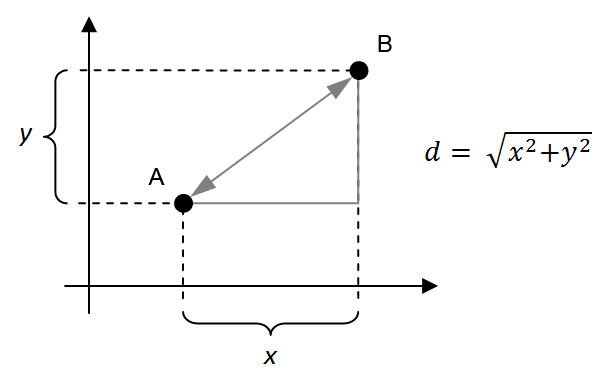
\includegraphics[scale=0.5]{obrazki/euklides}
  \caption{Przykład obliczania metryki eukliesowej.}
\end{figure}
\subsubsection{Metryka Manhattan}
\label{subs:Metryka Manhattan}
Metryka Manhattan, w której odległość dwóch punktów to suma wartości bezwzględnych różnic ich współrzędnych, zgodnie z poniższym wzorem:
$$d_m(x,y) = \sum\limits_{k=1}^n |x_k - y_k|$$
Przykład:
\begin{figure}[h]
  \centering
  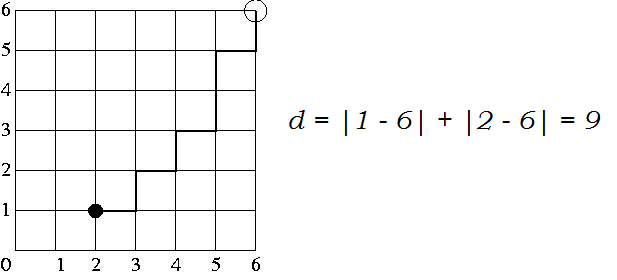
\includegraphics[scale=0.5]{obrazki/manhattan}
  \caption{Przykład obliczania metryki manhattan.}
\end{figure}

\section{Algorytm nearest neighbour}
\label{sec:Algorytm nearest neighbour}
Algorytm k-NN pozwala wyszukać w zadanym zbiorze punktów, k punktów znajdujących się najbliżej nowego punktu, korzystając przy tym z wybranej miary odległości.\\
W zagadnieniu klasyfikacji, algorytm k-NN przyjmuje jako argument tzw. zbiór uczący składający się z wielowymiarowych wektorów cech oraz przypisanych do nich klas. Faza klasyfikacji nowego obiektu polega na przypisaniu odpowiedniej klasy nieznanemu wektorowi cech. Nowy obiekt przypisywany jest do klasy, która występuje najczęściej wśród k najbliżej znajdujących się obiektów ze zbioru uczącego, zgodnie z wybraną metryką. Specjalnym przypadkiem algorytmu jest sytuacja, w której $k = 1$. Nazywa się algorytmem najbliższego sąsiada, w którym klasa nowego obiektu ustalana jest na podstawie najbliżej leżącej próbki ze zbioru danych uczących. Na poniższym rysunku przestawiona została przykładowa przestrzeń zawierająca dane uczące (niebieskie kwadraty oraz czerwona trójkąty) oraz niezidentyfikowaną próbkę – zielone kółko):
\begin{figure}[h]
  \centering
  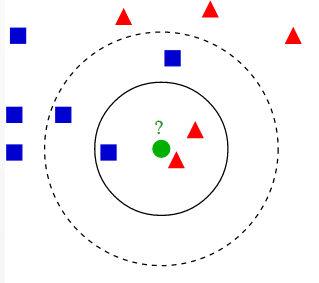
\includegraphics[scale=0.5]{obrazki/knn}
  \caption{Klasyfikacja w algorytmie k-nn.}
\end{figure}

Przyjmując liczbę najbliższych sąsiadów $k = 3$ (ciągła linia na rysunku),  nowy obiekt zostanie przypisany do grupy czerwonych trójkątów, ponieważ jest ich więcej wśród 3 najbliższych próbek. Przyjmując $k = 5$, nowy obiekt zostanie przypisany do klasy niebieskich kwadratów, ponieważ w najbliższym otoczeniu znajdują się 3 kwadraty i tylko 2 trójkąty.

\section{Algorytm nearest mean}
\label{sec:Algorytm nearest mean}
Algorytm nearest mean jest jednym z algorytmów minimalnoodległościowych. Jest on wykorzystywany w statystyce to prognozowania wartości pewnej zmiennej losowej bądź do zadania klasyfikacji.

Założenia:
\begin{itemize}
  \item dany jest zbiór uczący, który zawiera obserwacje. Każda z obserwacji ma przypisany wektor zmiennych objaśniających $X_1...X_n$ oraz wartość zmiennej objaśnianej $Y$,
  \item dana jest obserwacja $C$ z przypisanym wektorem zmiennch objaśniających $X_1...X_n$ dla której chcemy prognozować wartość zmiennej objaśnianej $Y$.
\end{itemize}

Przebieg algorytmu:
\begin{enumerate}
  \item korzystając ze zbioru uczącego oblicz centroid dla każdej wartości zmiennej objaśnianej $Y$,
  \item zaklasyfikuj obserwację $C$ do jednej z klas zmiennej objaśnianej $Y$ poprzez minimalizację odległości pomiędzy wektorem wybranych cech, a centroidem.
\end{enumerate}

\chapter{Implementacja}
\label{chap:Implementacja}
\section{Informacja o środowisku implementacyjnym}
\label{sec:Informacja o środowisku implementacyjnym}
Algorytmy zostały zaimplementowane w środowisku \textbf{MATLAB}. Ranking cech został uzyskany przy pomocy środowiska \textbf{Orange} (\url{http://orange.biolab.si/}). Jest to rozwiązanie open source, które umożliwia wizualizację oraz analizę~danych.
\section{Ranking cech}
\label{sec:Ranking cech}
Korzystając z narzędzia \textbf{Orange} wygenerowaliśmy ranking cech przedstawiony na rysunku \ref{fig:ranking}.
\newpage
\begin{figure}[h]
  \label{fig:ranking}
  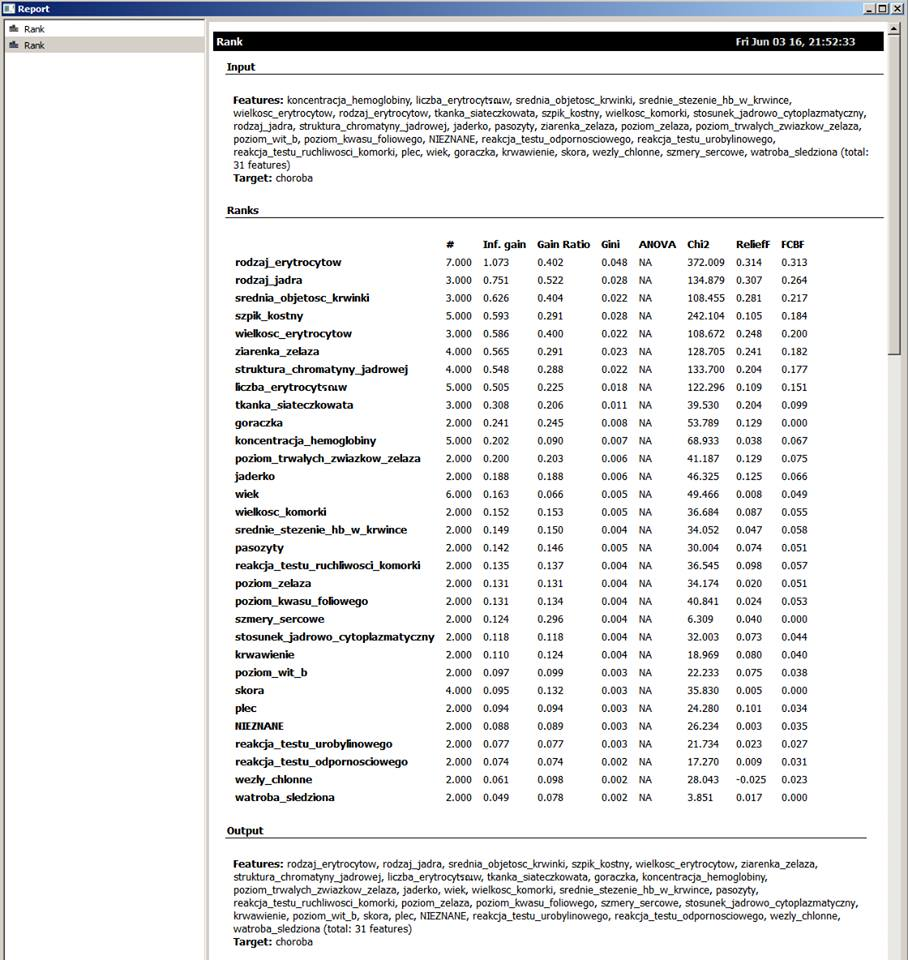
\includegraphics[scale=0.5]{obrazki/ranking}
  \caption{Ranking cech.}
\end{figure}

\section{Implementacja algorytmów}
\label{sec:Implementacja algorytmów}
\subsubsection{Nearest mean}
\label{subs:Nearest mean}
Na poniższych listingach przedstawione są najważniejsze części programów.

\begin{lstlisting}[label={lst:podzial},caption={Podział danych na zbiór uczący i testowy.}]
data = data(randperm(end), :);
train = data(1:floor(0.5*size(data, 1)), :);
test = data(floor(0.5*size(data, 1))+1:end, :);
\end{lstlisting}

\begin{lstlisting}[label={lst:centroidy},caption={Etap treningu - wyznaczanie centroidów.}]
centroid = [unique(data(:, 1)) zeros(size(unique(data(:, 1)), 1), size(data, 2)-1)];

for label = unique(train(:, 1))'
    % zbierz wszystkie próbki danej klasy
    train(train(:, 1) == label, 2:end)
    % oblicz centroid dla danej klasy
    centroid(centroid(:, 1) == label, 2:end) = mean(train(train(:, 1) == label, 2:end));
end
\end{lstlisting}

\begin{lstlisting}[label={lst:pre_result},caption={Wyznaczenie odległości próbki od centroida i przydzielenie do klasy.}]
pre_result = zeros(size(test, 1), 1);
for i = 1:size(test, 1)
    dist = pdist2(test(i, feature_rank(1:k)), centroid(:, feature_rank(1:k)));
    [~, templabel] = min(dist);
    pre_result(i) = centroid(templabel, 1);
end
\end{lstlisting}

\chapter{Opis badań eksperymentalnych}
\label{chap:Opis badań eksperymentalnych}
Badania eksperymentalne zostały przeprowadzone zgodnie z instrukcją. Zastosowano trenowanie i testowanie klasyfikatorów z wykorzystaniem 5 razy powtarzanej metody 2-krotnej walidacji krzyżowej. Zastosowane miary odległości to miara euklidesowa i Manhattan.
\section{Wyniki badań}
\label{chap:Wyniki badań}
\subsection{Algorytm nearest mean}
\label{subs:Algorytm nearest mean}
Wyniki badań dla algorytmu nearest mean zostały przedstawione na rysunku \ref{fig:nm_res}.

\begin{figure}[h]
  \centering
  \label{fig:nm_res}
  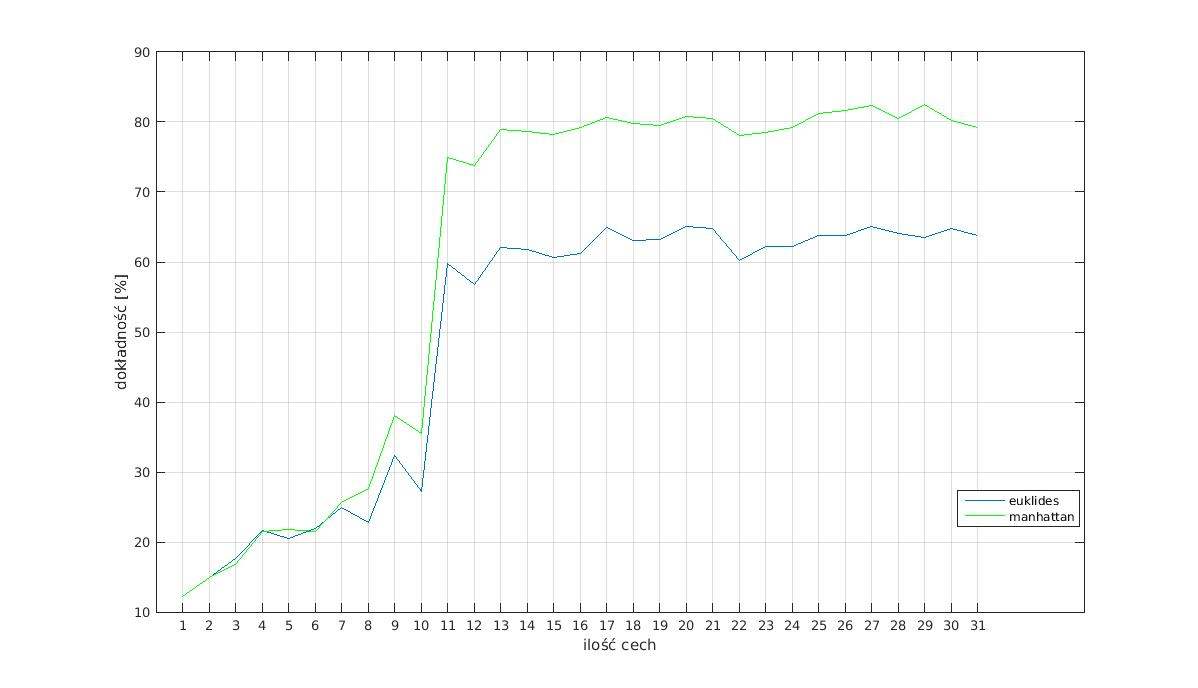
\includegraphics[scale=0.4]{obrazki/nm_plot}
  \caption{Wynik badań dla algorytmu nearest mean.}
\end{figure}

Jak widać na rysunku, dokładność klasyfikacji rośnie wraz ze zwiększaniem liczby cech biorącej udział w klasyfikacji. Największy skok dokładności występuje przy wykorzystaniu 11 cech (różnica na poziomie 40\%). Kolejne zwiększanie ilości cech utrzymuje dokładność klasyfikacji na względnie równym poziomie (nie ma dużych wzrostów ani spadków dokładności klasyfikacji).\\
Z rysunku można również odczytać, że wpływ na dokładność klasyfikacji ma wybrana metryka. Od momentu dołożenia 11 cechy, czyli największego wzrostu dokładności klasyfikacji, klasyfikacja dla metryki euklidesowej jest średnio 25-30\% gorsza od metryki Manhattan.

\chapter{Podsumowanie i wnioski}
\label{chap:Podsumowanie i wnioski}
\section{Wnioski płynące z analizy wyników}
\section{Ocena krytyczna i podsumowanie projektu}

\begin{thebibliography}{}
\addcontentsline{toc}{chapter}{Bibliografia}
\bibitem{1}
M.M. Sysło, N.Deo, J.S. Kowalik, \textit{Algorytmy optymalizacji dyskretnej z programami w języku Pascal}, Wydawnictwo Naukowe PWN , 1999

\bibitem{2}
R. Neapolitan, K. Naimipour, \textit{Podstawy Algorytmów z przykładami w C++}, Helion, 2004

\bibitem{3}
T. H. Cormen, C. E. Leiserson, R. L. Rivest, C. Stein, \textit{Wprowadzenie do algorytmów}, Wydawnictwo Naukowe PWN, 2013

\end{thebibliography}
\end{document}
